The final stage is the classification stage. The inputs to this stage are the max-pooled masked images and feature vectors described in section \ref{preprocessing}. However, instead of using this as a direct input for classification, we reduce this data further as our objective is to reduce computational complexity and get a good runtime.

Principal component analysis (PCA) is a data transformation technique used to reduce the dimensionality of high-dimensional data into a low-dimensional subspace while maintaining most of the variance \cite{b5_1,b5_2}. We use PCA to reduce the inputs to maintain 95\% of the variance. The reduced data is used as the input for classification as illustrated in Fig. \ref{fig:pca}.

We investigate using two different ensemble classifiers to compare accuracy. The ensemble method is a powerful technique that combines multiple models into a single predictive model. This often makes it more accurate and reliable than its individual components \cite{b5_3}. The first classifier we use is a decision tree classifier wrapped in a bagging based ensemble model. The bagging method selects a random subset of the dataset with replacements for training each model and uses a voting scheme to make a final prediction \cite{b5_4}. One of the more prominent examples of a bagged decision tree model is random forest \cite{b5_5}.

The second classifier we use is a support vector machine (SVM) classifier in a boosting based ensemble model. The boosting method selects a subset of the dataset without replacements for training individual models \cite{b5_6}. By focusing on the incorrect classifications, it adjusts the weights of each model's prediction and produces a final prediction that is a weighted avergage of the individual predictions. We use SVM for the classifier as it is considered to be one of the best machine learning classification and regression techniques capable of classifying large datasets with high accuracies \cite{b5_7,b5_8,b5_9}.

\begin{figure}[tp]
	\centerline{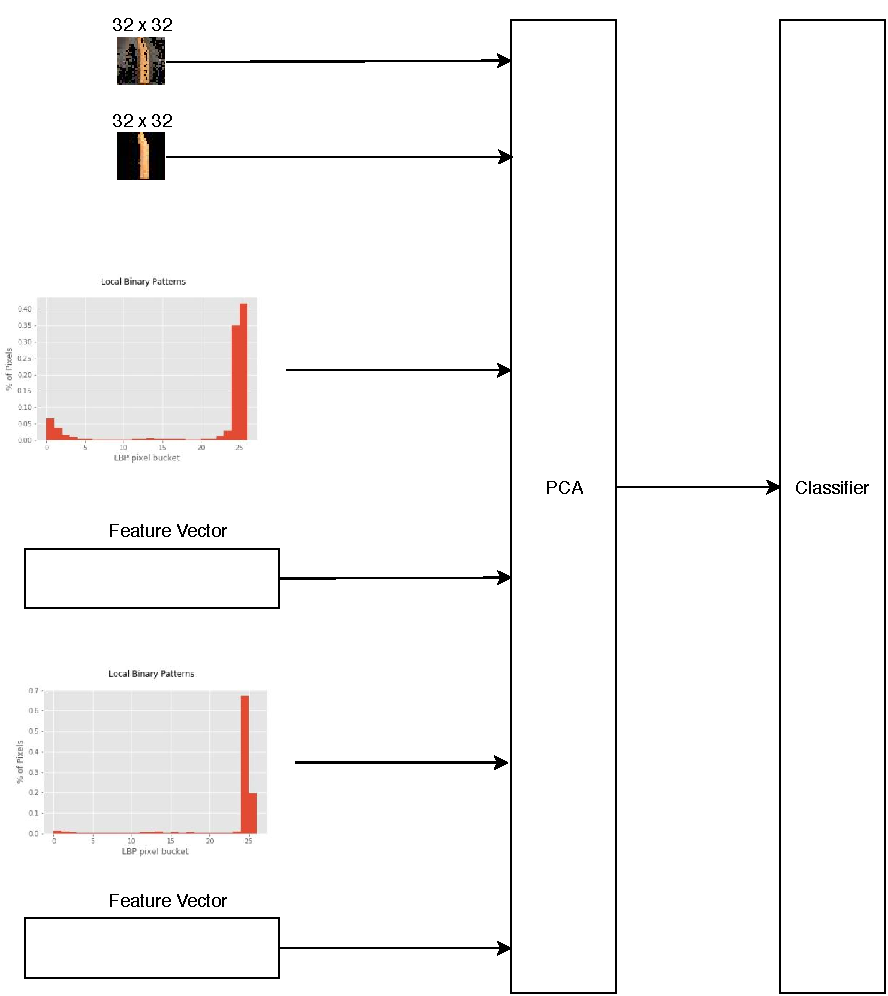
\includegraphics[scale=0.5]{./img/pca.pdf}}
	\caption{The steps to transform the input before classification.}
	\label{fig:pca}
\end{figure}